\chapter{Diagramas de secuencia}

\section{Cargar XML}

\begin{figure}[H]
\centering
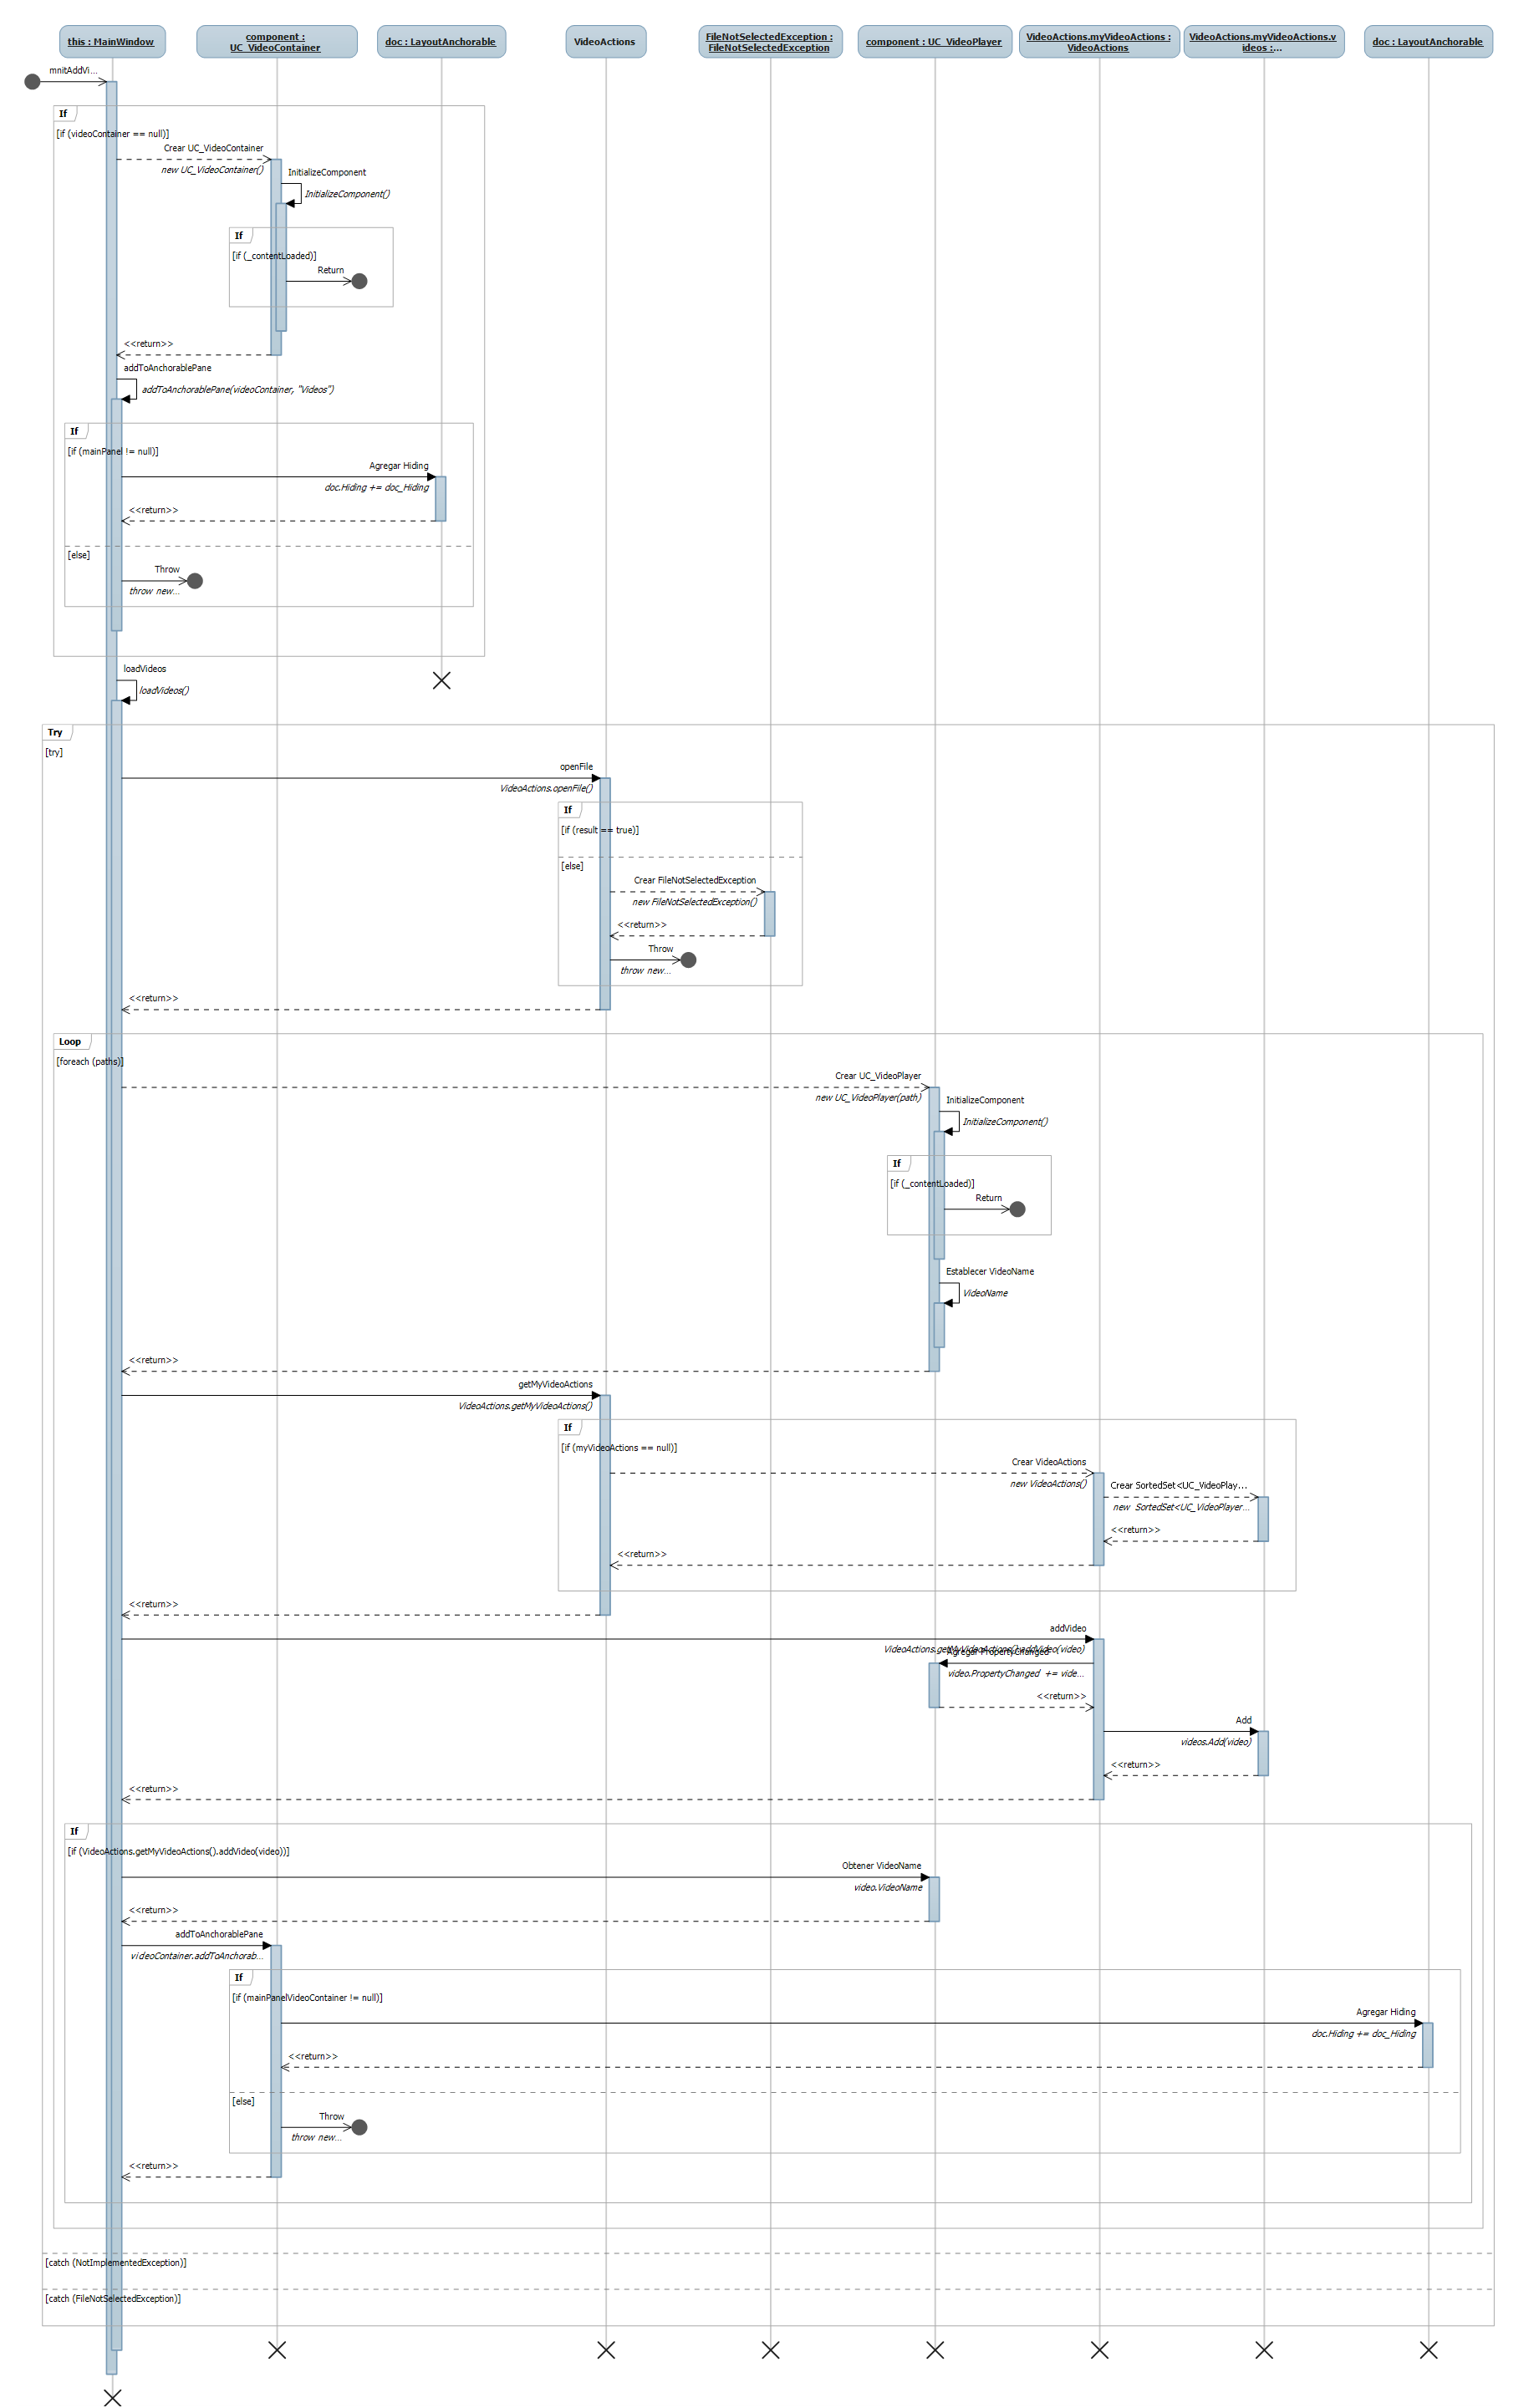
\includegraphics[width=0.6\linewidth]{./Figures/Secuencia/CargarXML.png}
\caption{Cargar XML}
\label{fig:CargarXML}
\end{figure}


\section{Cargar observaci\'on o propiedad}

\begin{figure}[H]
\centering
\includegraphics[width=0.7\linewidth]{./Figures/Secuencia/LoadObservationProperty}
\caption{Cargar observaci\'on o propiedad}
\label{fig:LoadObservationProperty}
\end{figure}


\section{A\~nadir v\'ideo}
\begin{figure}[H]
\centering
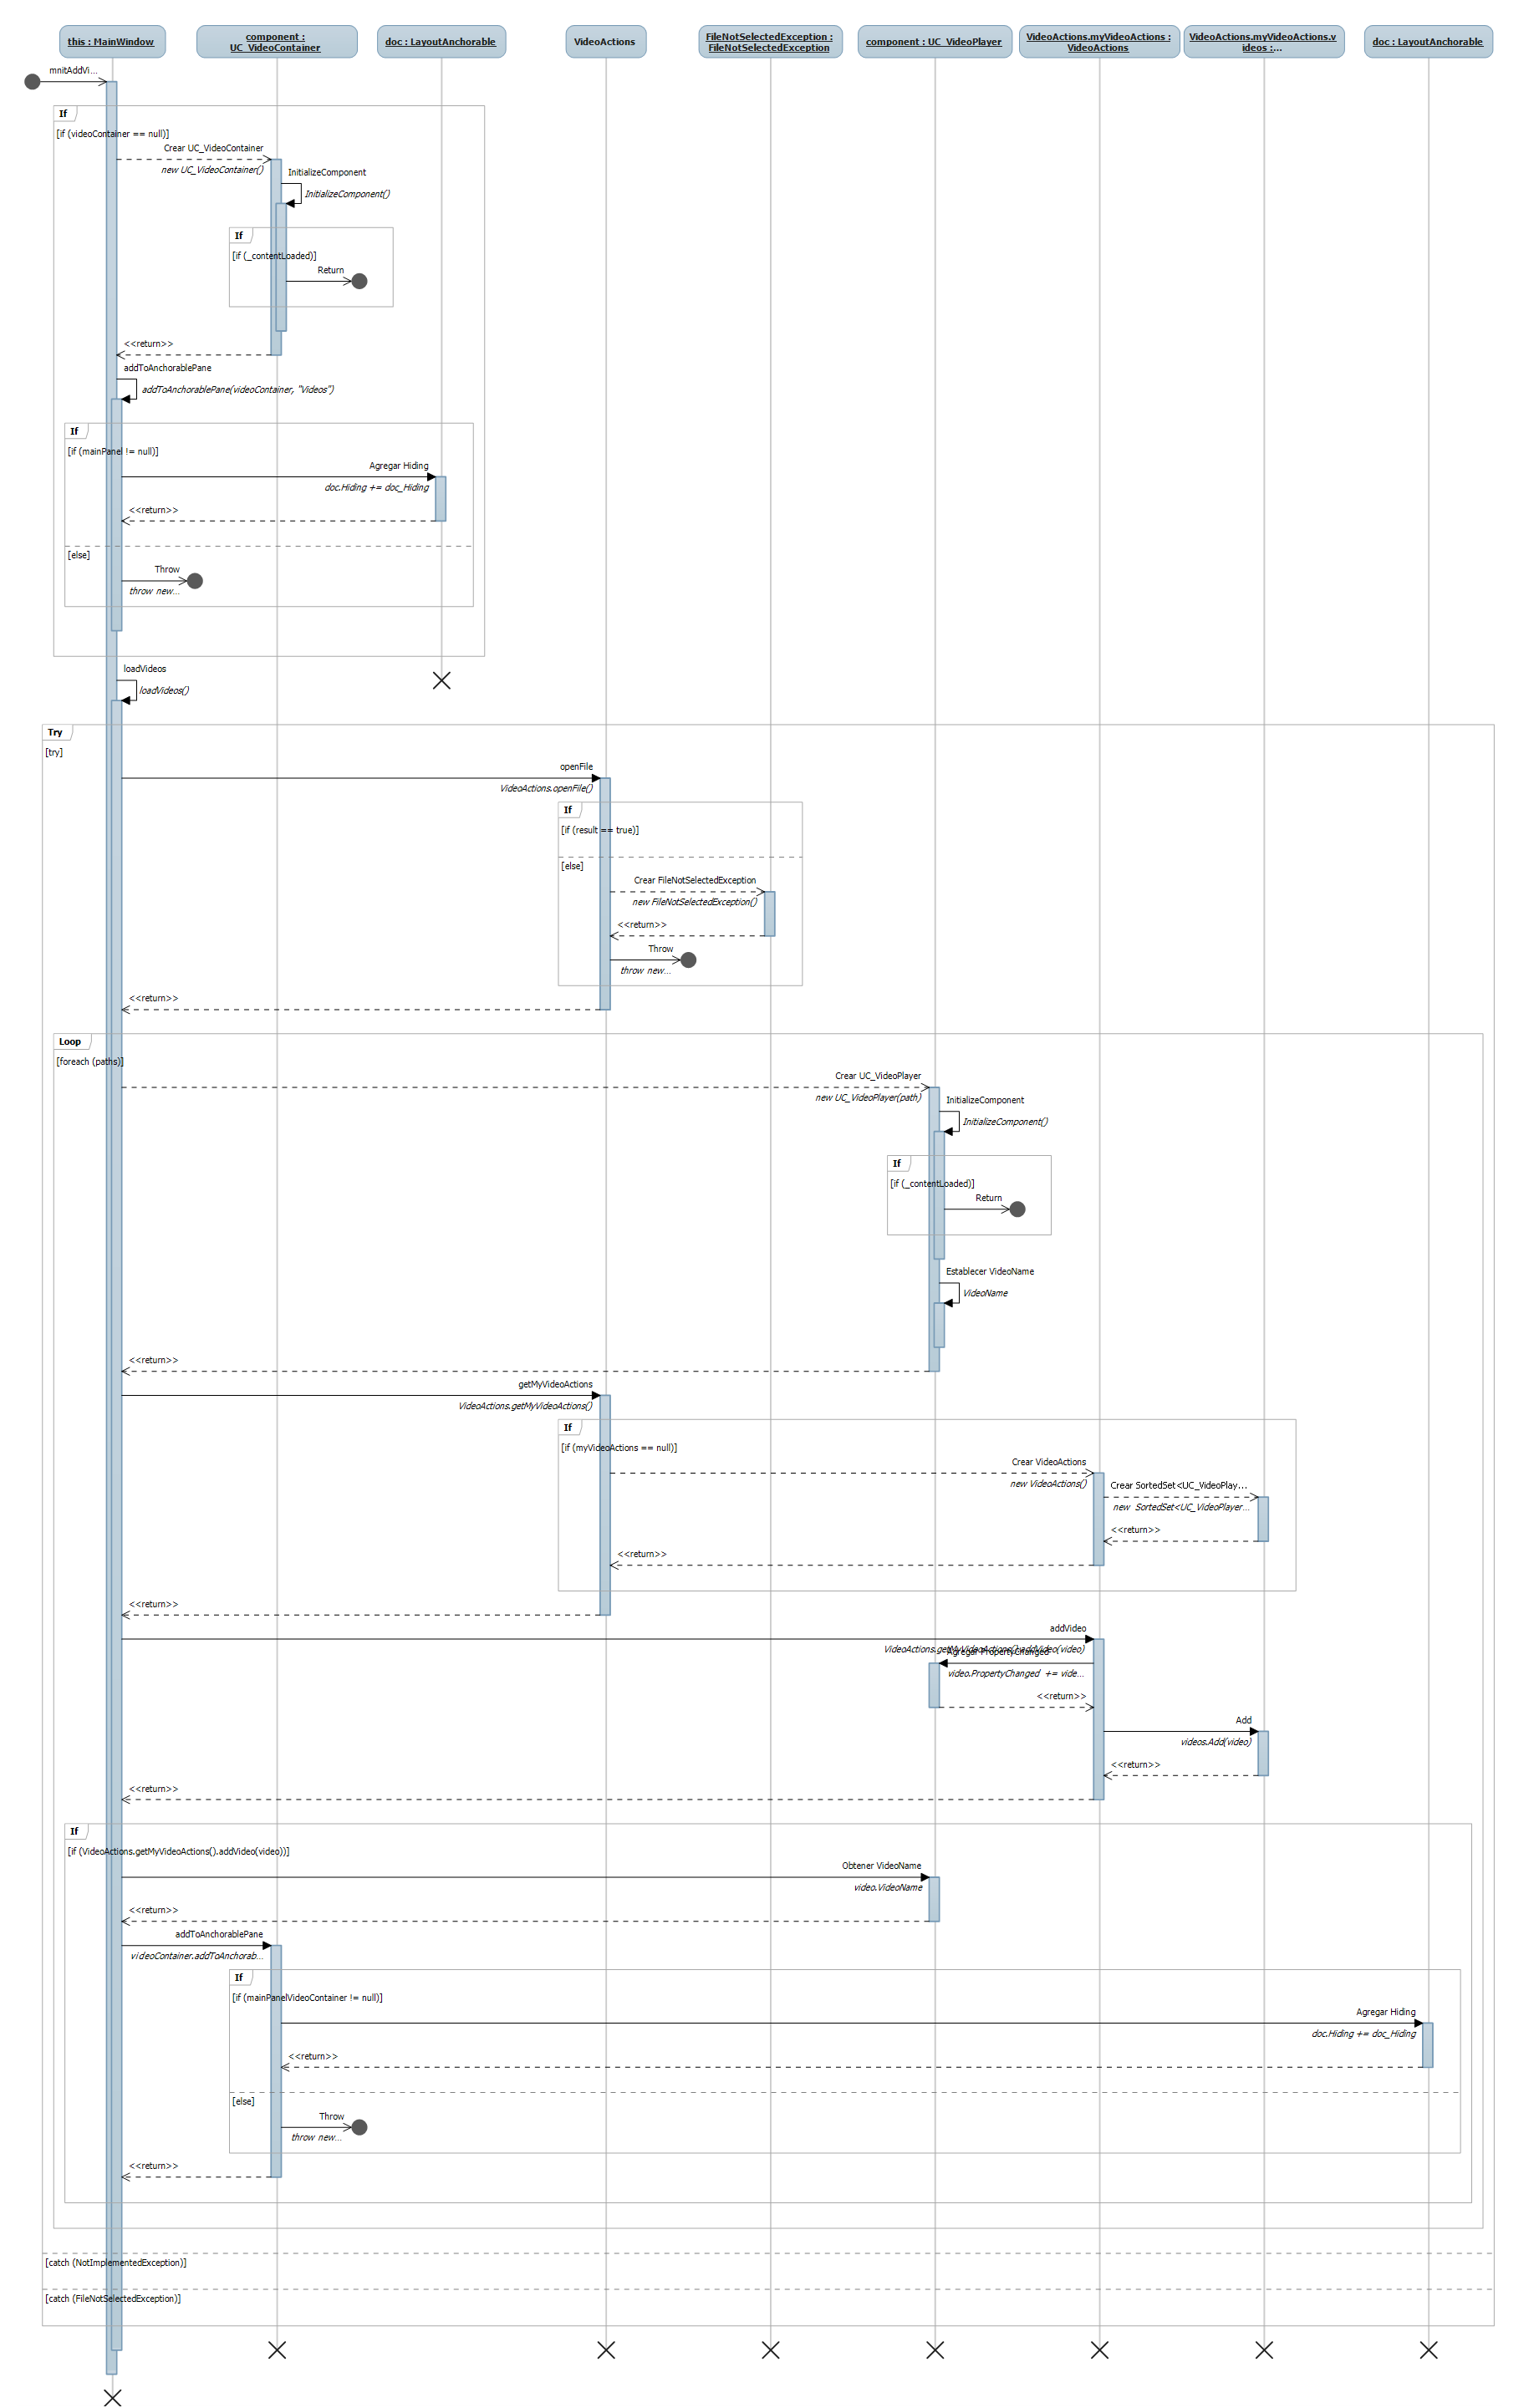
\includegraphics[width=0.8\linewidth]{./Figures/Secuencia/AddVideo}
\caption{A\~nadir v\'ideo}
\label{fig:AddVideo}
\end{figure}

\section{Crear intervalo}
\begin{figure}[H]
\centering
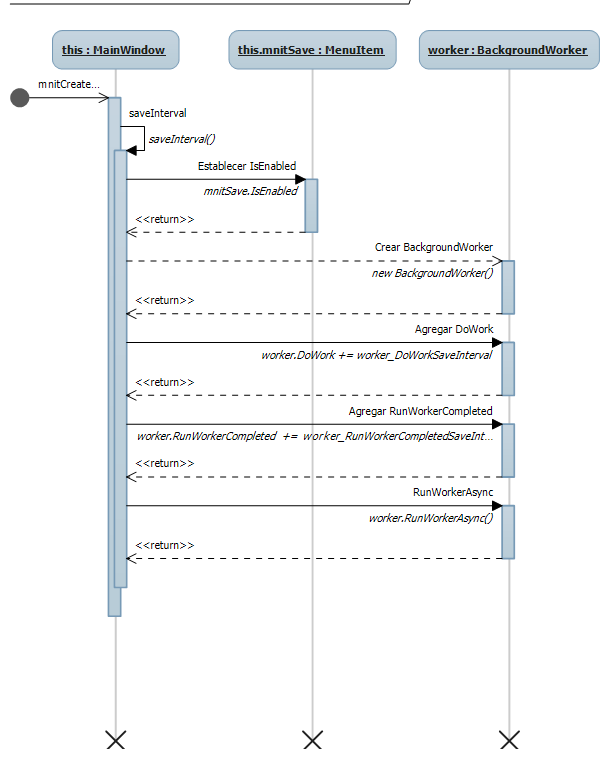
\includegraphics[width=0.9\linewidth]{./Figures/Secuencia/CreateInterval}
\caption{Crear intervalo}
\label{fig:CreateInterval}
\end{figure}

\begin{figure}[H]
    \centering
    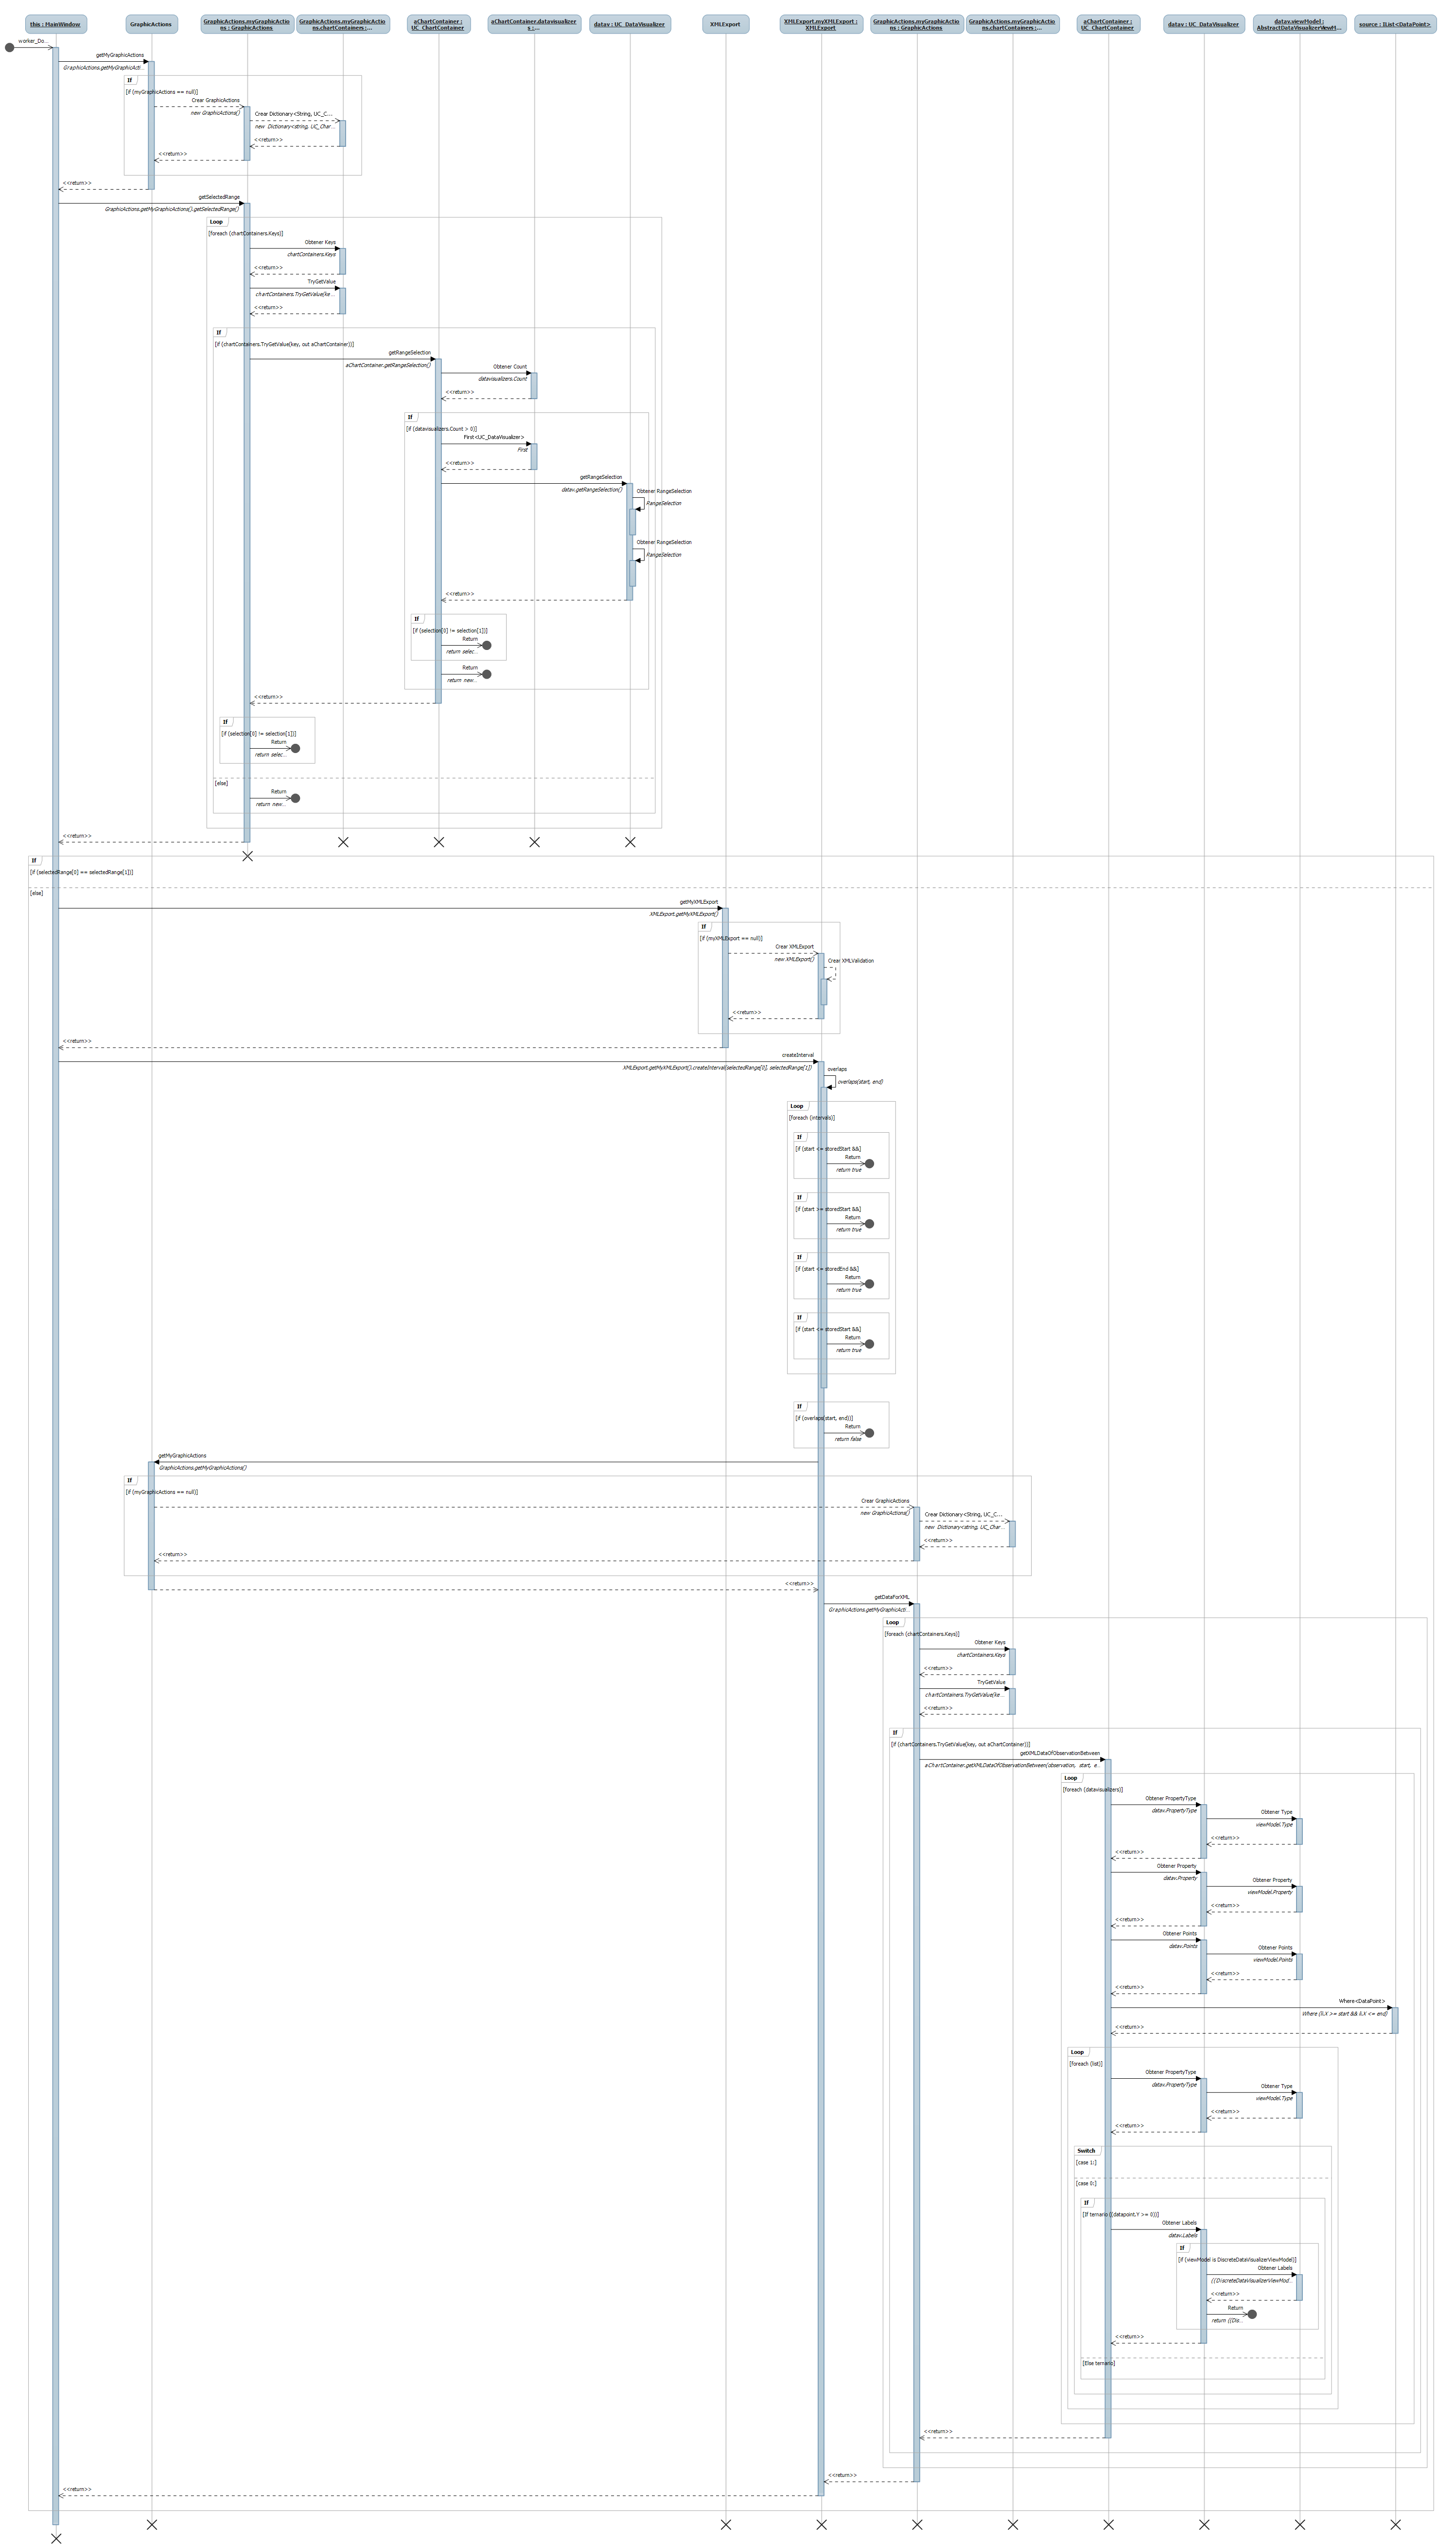
\includegraphics[width=0.8\linewidth]{./Figures/Secuencia/CreateIntervalWorker}
    \caption{Crear intervalo, parte del worker}
    \label{fig:CreateIntervalWorker}
\end{figure}

\section{Seleccionar rango}
\begin{figure}[H]
\centering
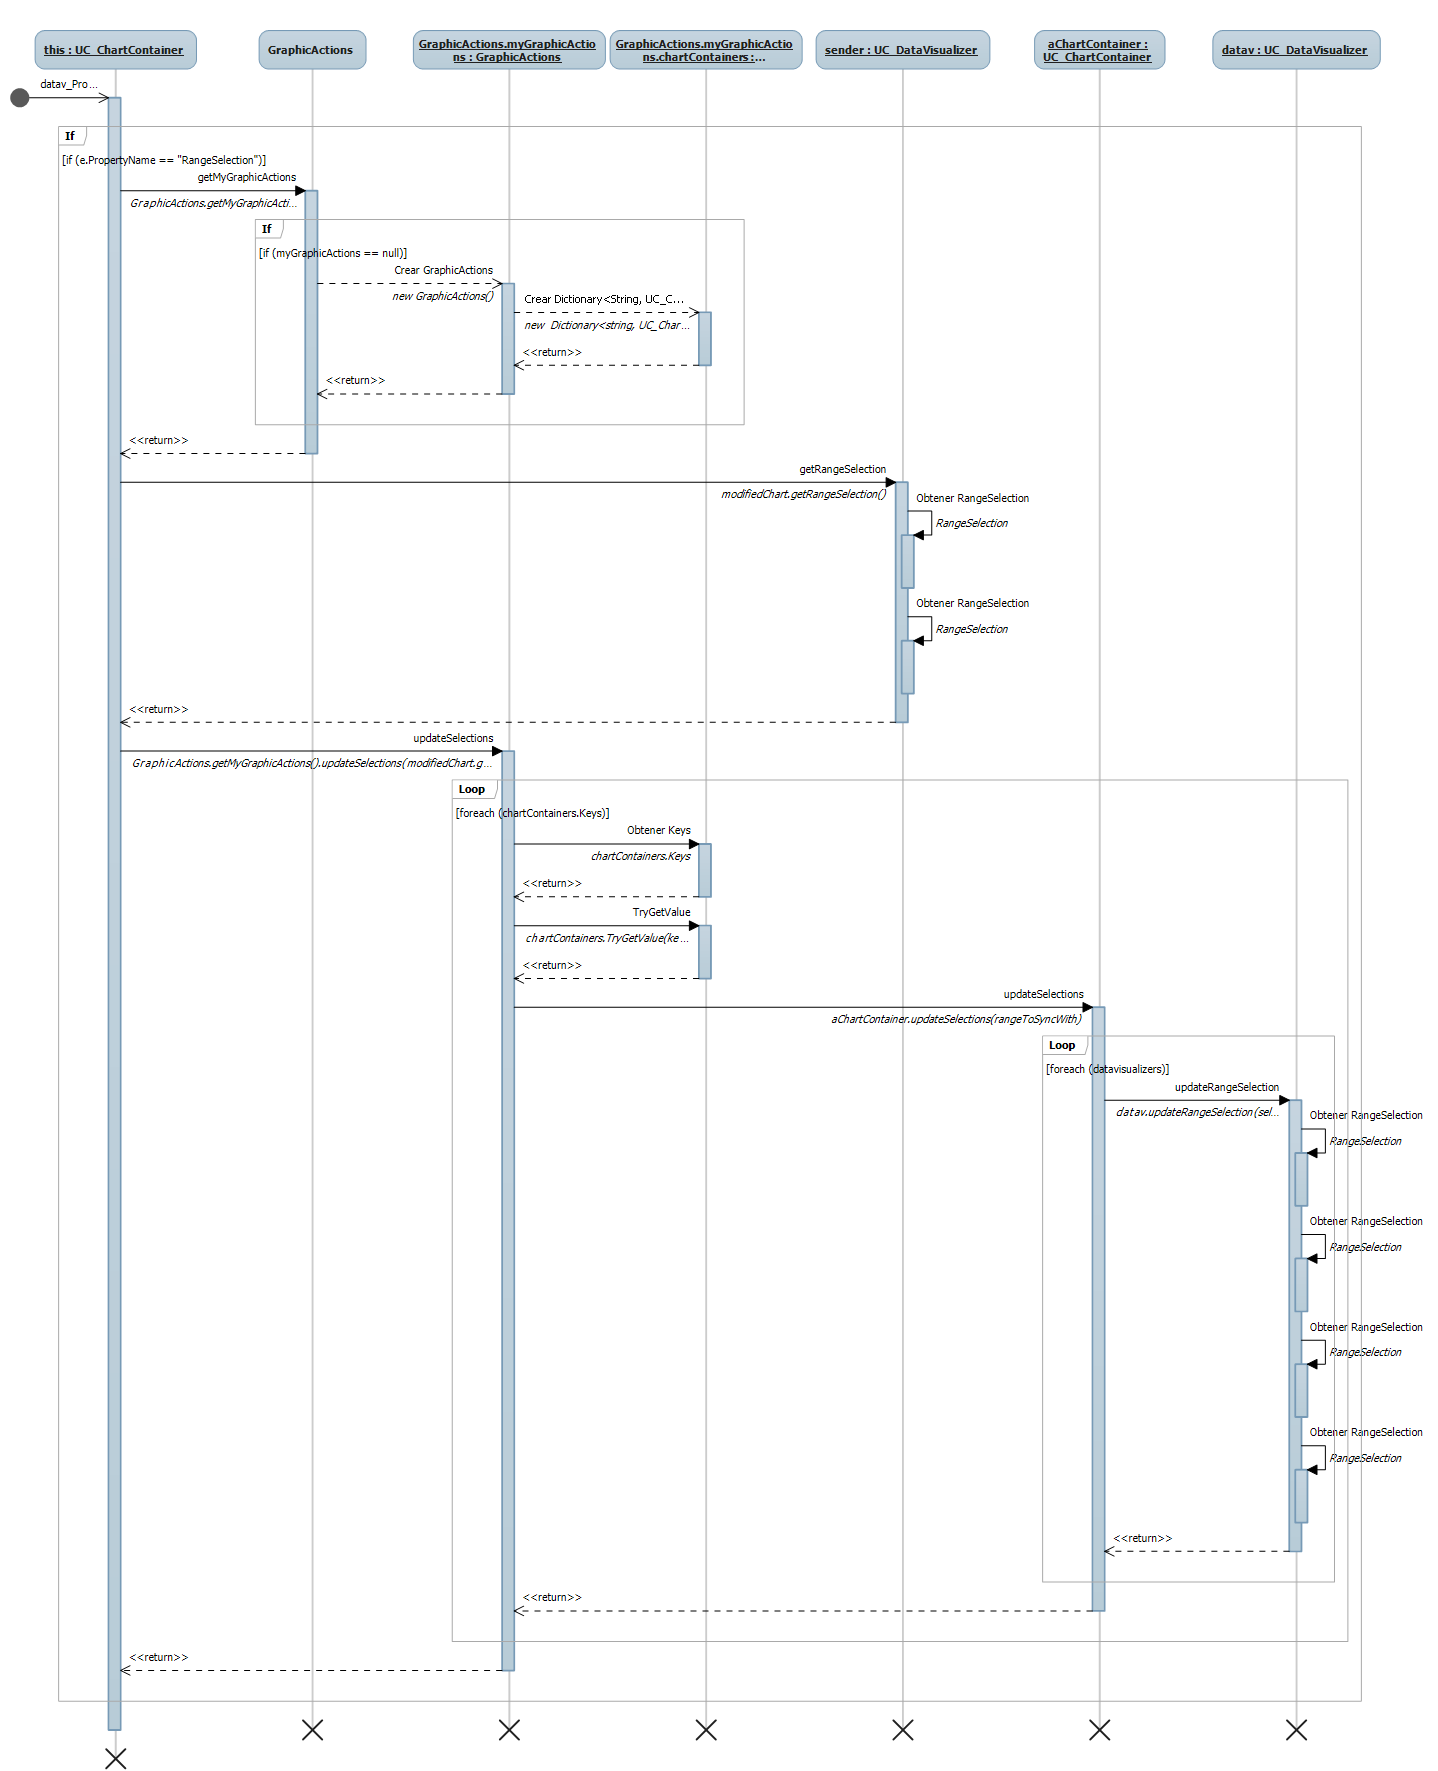
\includegraphics[width=0.9\linewidth]{./Figures/Secuencia/RangeSelectionPropertyChanged}
\caption{Seleccionar rango}
\label{fig:RangeSelectionPropertyChanged}
\end{figure}

\section{Guardar paso o situaci\'on}
\begin{figure}[H]
\centering
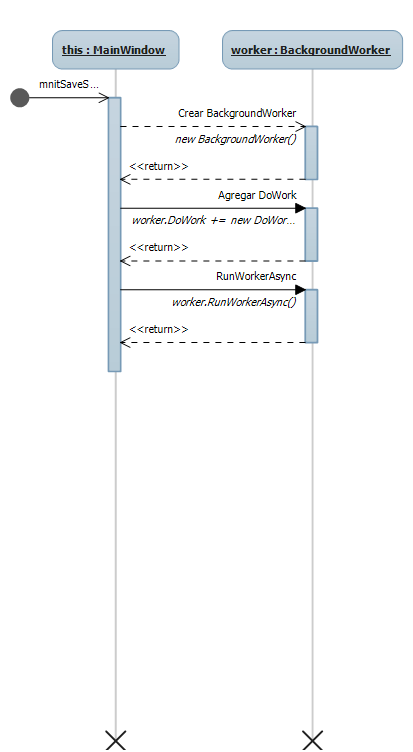
\includegraphics[width=0.7\linewidth]{./Figures/Secuencia/SaveStepSituation}
\caption{Guardar paso o situaci\'on}
\label{fig:SaveStepSituation}
\end{figure}

\begin{figure}[H]
\centering
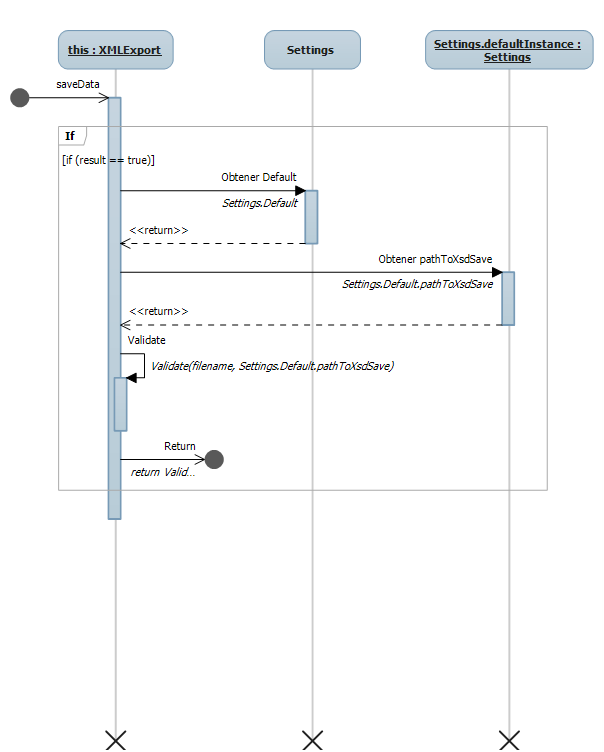
\includegraphics[width=0.7\linewidth]{./Figures/Secuencia/XMLExportSaveData}
\caption{Guardar paso o situaci\'on, parte worker}
\label{fig:XMLExportSaveData}
\end{figure}
